\chapter{Overview\label{chap2}}
A comprehensive overview of the project is given in this chapter. Firstly, an in-depth examination of the five given tasks is made. In the second part of this chapter, we briefly describe our designing workflow for dealing with these  tasks. Then we introduce our proposed solutions under the guidance of it.
\section{Project Overview\label{sec2.1}}
\begin{figure}[htbp]
    \centering
    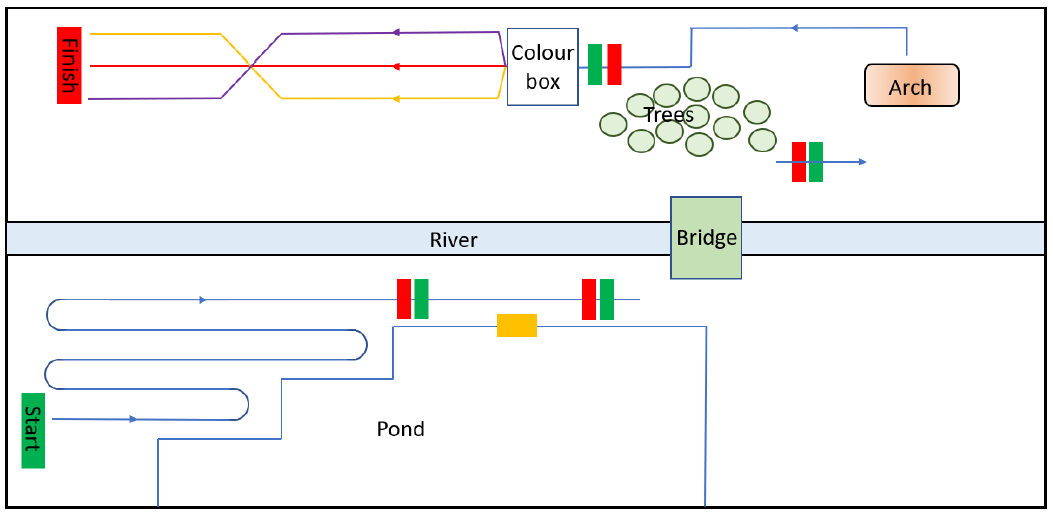
\includegraphics[width=15cm]{overview/img_overview/patio.png}
    \caption{Five tasks marked by Green and Red boxes}
    \label{fig:patio}
\end{figure}
According to the course specifications, our proposed design is expected to accomplish the following five tasks. In the first task, the rover starts from the green box as indicted in Figure \ref{fig:patio} and then move along the lines  until it reaches the first red box. The second task is from the second green box to the second red box, between which the rover should recognize the orange fish tank and drop the fish food right onto it. In the next task, the rover is expected to move autonomously, crossing the bridge and turning right before crashing into the forest. Then, the rover should pass the arch and then follow the lines to the starting point of the Task 5, where the rover is required to recognize the color of a randomly initialized color box, and follow the path with the same color till the red box 
at the end.\footnote{Note: The green and red boxes are only for illustration. They do not really exist in our design}



There are some specific requirements for this project, which are listed in Table \ref{tab:project_specifications}.

\begin{table}[htbp]
    \centering
    \begin{tabular}{lll}
    \toprule
    \textbf{Object}  & \textbf{Specification} & \textbf{Note}                           \\
    \midrule
    patio   & 100 m  $\times$ 30 m            &  length $\times$ width                  \\
    rover   & 50 cm $\times$ 50 cm            & maximum size                            \\
    bridge  & 100 cm $\times$ 3 m             &  width $\times$ length                  \\
    arch    & 100 cm $\times$ 100 cm          &  width $\times$ height (suggested size) \\
    beacon  & no more than 2                  &                                         \\  
    sensor & no number limitations            &                                         \\
    \bottomrule
    \end{tabular}
    \caption{The project specifications}
    \label{tab:project_specifications}
\end{table}

\section{Designing Workflow}
During the project development, we adopt an interactive designing strategy. The whole process is shown in Figure \ref{fig:development strategy}. Both the Visual and the Chassis Group firstly search for possible solutions and have them examined by the Decision Group. The Decision Group then choose optimal ones from them and split the whole project into small achievable subtasks. If the provided solution does not fit the requirement of the Decision Group, it will be rejected and modifications will be made to improve it. Our program is developed with Python.

\begin{figure}[htbp]
    \centering
    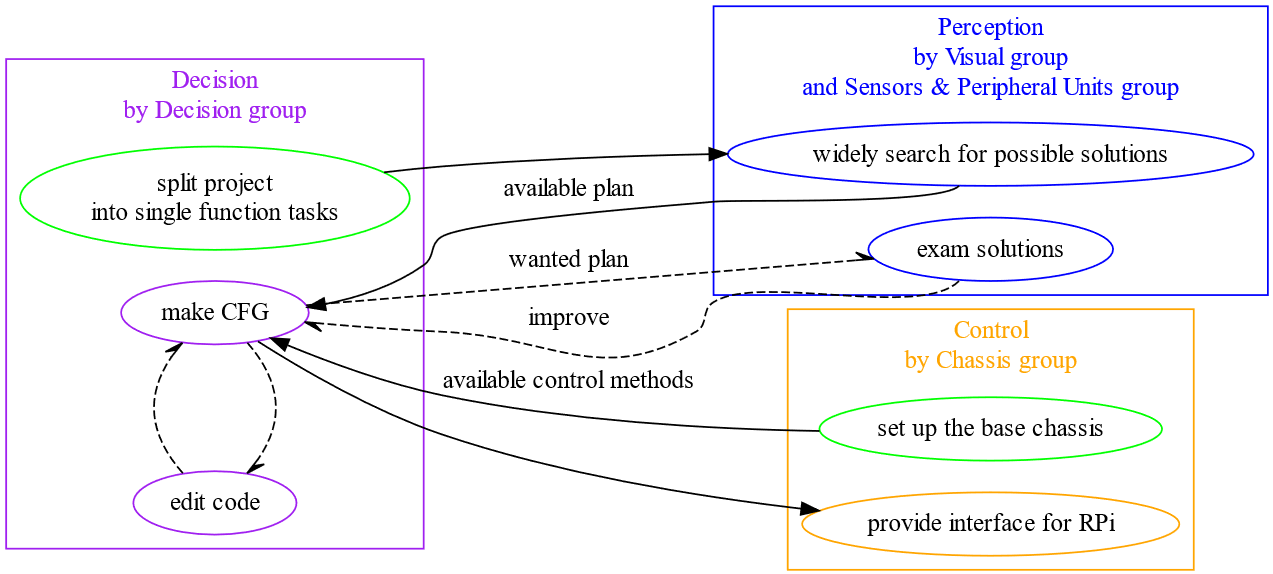
\includegraphics[width=12cm]{overview/img_overview/development_strategy.png}
    \caption{The development strategy}
    \label{fig:development strategy}
\end{figure}

With a joint effort of the three main groups, an overall design is finally made. Here, we introduce it task by task.
\begin{itemize}
    \item \textbf{Task 1:} When the path camera identifies the path, a “Path\_Direction” signal of the angle between the car and the path direction could be sent from visual group to decision group. Then, a “Turn” command with the angle are sent from decision group to chassis group, leading the car to drive following the line.
    \item \textbf{Task 2:} When the path camera recognizes the orange box, the “Beacon” signal which is “tank” will be sent to decision group. The bool “isFeeded” turn to True to promise the “Feed” command could only be sent to chassis group for one time.
    \item \textbf{Task 3:} When the line cannot be found for more than 7 second, the “Path\_Direction” signal will be replaced by “Direction\_x”, the angle between the car and x axis, which is measured by compass. After the left camera identifies the bridge at the center of view, the “Direction\_x” signal will be replaced by “Direction\_-z”, leading the car turn to aim to the bridge. The, the “Turn” command with the angle with z axis are sent together to chassis group, helping the car crosses the bridge along z axis. After the path camera recognizes the green beacon behind the bridge, the “Beacon” signal which is “after bridge” will be sent to decision group. Then, the “Direction\_x” signal takes place of “Direction\_-z”. As a result, the car could run along x axis again.
    \item \textbf{Task 4:} When the left camera identifies the gate at the center of view, the signal “Gate\_Direction” could be received by decision group. “Turn” command with the angle of “Direction\_-z” are sent together to chassis group in order to let the car turn to the gate and drive ahead to cross it. After crossing the gate, the line can be seen again by the path camera. Therefore, the “Path\_Direction” signal leads the car again to drive along the line.
    \item \textbf{Task 5:} When the car drive to the start of color line, it recognize its color first. Then we filter input images from the path camera by preserving this color only. In this way, this task could be simplified like the Task 1. Although the line may be separated at the intersection, we use the lost\_count signal to count for 7 seconds to ensure the car can keep driving along the line until it reaches the real finish position.
\end{itemize}

